\documentclass{article}

\usepackage[parfill]{parskip}
\usepackage{graphicx}
\usepackage{booktabs}

\title{AutoRSpec}
\date{2017-04-25}
\author{Dan Shreeve}

\begin{document}

\pagenumbering{roman}
\addcontentsline{toc}{section}{Title page}
\maketitle

\newpage
\addcontentsline{toc}{section}{Signed declaration}
\section*{Signed declaration}
All sentences or passages quoted in this report from other people's work have been specifically acknowledged by clear cross-referencing to author, work and page(s). Any illustrations which are not the work of the author of this report have been used with the explicit permission of the originator and are specifically acknowledged. I understand that failure to do this amounts to plagiarism and will be considered grounds for failure in this project and the degree examination as a whole.
\par Name: Daniel Demaine Shreeve
\par Signature: .................................
\par Date: 03/05/2017

\newpage
\addcontentsline{toc}{section}{Abstract}
\begin{abstract}
Software Testing benefits the development and maintenance of a system by increasing quality and reliability. Software Testing also contributes around half of the cost of producing a system. Automating part or whole of this process reduces the cost while maintaining the benefits. The aim of this project is to produce a system that automatically generates RSpec test cases for model validation in Ruby on Rails. The tests will be generated from a formal database specification that the user has defined using the system. A file can be generated and inserted into the users application and run as though they been written by the user. The time taken to insert the information should be less than the time taken to write the tests manually, otherwise the user does not benefit.
\end{abstract}

\newpage
\addcontentsline{toc}{section}{Acknowledgements}
\section*{Acknowledgements}
First and foremost I would like to thank my supervisor \textbf{Dr. Gordon Fraser} for accepting my proposed project and providing impeccable advice and guidance throughout the process.
\par Finally I would like to thank my parents, \textbf{Linda Shreeve} and \textbf{Paul Shreeve}, and my grandparents \textbf{Elsie Marsden} and \textbf{Ray Marsden} for giving me the oppurtunity to go to university and supporting me throughout.

\newpage
\tableofcontents

\newpage	
\pagenumbering{arabic}
\section{Chapter 1: Introduction}


\subsection{Importance of Testing}

\par How severe can the consequences be from an error in a piece of software? In 1983 a bug in a piece of software nearly started World War Three.
\vspace{5mm}
\par During the Cold War, tensions between the US and Soviet Russia were extremely high. A Soviet early warning system had detected the launch of five ballistic missiles from the US. The only reason that Soviet Russia did not retaliate, starting World War Three, was the fact that Lt Col Stanislav Petrov had a "...funny feeling in my gut"\cite{ZDNetDisasters} and concluded that if the US was launching a full scale attack they would launch more than five missiles. The error in the system was discovered to be a bug in part of the software that distinguished false missiles from satellites picking up the reflection of sunlight from the top of clouds.\cite{ZDNetDisasters} If the bug in the code has falsey detected more missiles the world could be a very differn't place today.
\vspace{5mm}
\par  Software disasters are caused by three main reasons. Poor software project management, poor risk assessment and poor development and testing practices.\cite{mcquaid2012software} Software testing is therefore extremely prevelent and has upmost importance as it can prevent World War and save companies a lot of money.

\subsection{Benefits of Testing and Automation}

\par Inadequate software testing infastructure was estimated to cost the US economy \$59.5 billion a year.\cite{NISTReport} It was also estimated that the potentail cost reduction from feasbile infastructure would be \$22.2 billion a year. \cite{NISTReport} Due to software disasters and the vast amount of money that can be saved and also avoid incurring additonal costs, people have become more aware of the importance of testing. The benefits of the reduced costs  comes from ihe increased reliabilty and quality of the product produced when software testing is implemented.

\par "In a typical programming project approximately 50 percent of the elapsed time and more than 50 percent of the total cost were expended in testing the program or system being developed"\cite{myers2011art}. Software testing saves you alot of money but also costs alot of money. By automating part or the whole process the costs can be reduced while still obtaining all of the benefits.

\subsection{Ruby on Rails}
\par Ruby on Rails as a framework 
\par model as mvc
\par Rspec to test m

\subsection{Project Aims}
\par The overall aim of this project is to reduce the cost of developing Ruby on Rails applications. The reduction in costs comes from the time saved by automatically generating test cases for the model component of the application. The develop will input a formal specification of thier database into a system from which they can download seperate files containing a test suite for each table they have defined. The files are seperated in keeping with standard Ruby on Rails practices. Once the file is downloaded it can be inserted into the application and be available to run immediatley. This project should reduce the errors and bugs in Ruby on Rails applications via the feedback from the tests generated, improving the reliablity and quality of Ruby on Rails projects via the model component.



\subsection{Project Limitations}

\par Rails and its do more with less, inline with automated testing..

\par The aims of the project are to:
\begin{enumerate}
\item Reduce the amount of time it takes for a User to produce tests for model validation
\item Produce tests that are of high readable quality
\item Produce tests that fully test properties specified
\item The process should be hassle free
\end{enumerate}

\par Challenges that the project faces are
\begin{enumerate}
\item Identifying the minimum information required to produce tests
\item Creating a process that is hassle free
\item Natural language in tests that is appears human written
\item Generating the tests in an acceptable time frame
\item Building an efficent database structure for the information
\end{enumerate}


\section{Chapter 2: Literature Review and Research}

\subsection{Tools to use}
\par add a bit about bootstrap
\par The main requirements for choosing what tools to use to build the application are:
\begin{enumerate}
\item Allowing a User to enter information onto a database
\item Allowing a User to view information on the database
\item A system that can process the information and generate Test cases
\end{enumerate}
\par An MVC web application fits all these criteria while providing additional benefits. MVC, Model-View-Controller is an architectural pattern that seperates an application into three interconnected parts. The separation allows for responsibilities to be allocated independently to each component, seperating the logic from the user. The model is responsible for the data of the application and the rules and logic used to create and update the information. The view is responsible for displaying the data and possible interactions with the system to the user. The controller is responsible for controlling the flow of the system,  accepting user input and converting it into commands for the model and view.
\par An example of the components interacting would be creating an entry to a database. The view would be responsible for displaying the form in which to fill in. On submission the controller will process the information, ensure only persmissable information is submitted and enter additional information, then send it to the model. The model would verify the structure of the information, correct fields are present and cohere with its rules. The model will then notify the controller if the submission was successful or not and the controller will update the view to reflect the status.
\par The seperation means that all user interaction with the database has to be verified by the controller. This provides a high level of security as each action is controlled and the internal structure and representation of the information within the database is hidden. Simultaneous development is also possible due to the seperation of the components, work on the front and back end concurrently. Although I will not be able to get the full benefit of this as I am developing the project solo, it will allow me to shift focus as components do not need to finished before switching to another, giving greater flexibility in development. 
\par High levels of cohesion are inherited automatically from the architecture with the grouping of logically similar elements, this makes the code easier to read and creates a more natural flow within the source code. There are however some drawbacks to MVC architecture, they are inheritly more complex due to the seperation and the framework must be learnt in addition to the programming language it is in, which there can be multiple languages between the components. This steep learning curve could mean a large initail investment into a team learning a new framework along with its languages.
\par MVC web application frameworks have become extremely popular and are behind some of the most used and powerful websites. Django an MTV, follows MVC architecture but its creators decided to rename the components \cite{Django} to better suit them, is behind the two most visted websites in the world Google and YouTube\cite{SHUUP}\cite{Alexa}. Ruby on Rails another MVC is behind Twitter, Airbnb and Soundcloud.\cite{Coderfactory} MVC frameworks are known for their scalablity, being suitable for the smallest to the largest projects. However FaceBook decided that its scalablity had reached its limit, that adding new features made the code exponentailly more complex.\cite{Infoq} My project will be no where near the scale of facebooks sourcecode so I do not need to worry about reaching the end of its scalibilty.
\par The chosen MVC to construct the project in is Ruby on Rails. I have done previous projects in both Ruby and the Rails framework, also the novelty of contstructing the software in the software that its output will test.
\par Ruby was selected as the primary programming language by default as it is the language that runs Ruby On Rails. Ruby is a dynamic, multi-paradigm programming language. The paradigms consist of Object-oriented, Imperative, Functional and Reflective making it a very powerful and versatile language. This combination is from its founder ‘Yukihiro Matsumoto’ who was influenced by Perl, Smalltalk, Eiffel, Ada, and Lisp.
\par Ruby’s primary design goal was to “make a language that he himself enjoyed using, by minimizing programmer work and possible confusion”(Ruby Wiki). Achieved with a focus on human interaction, how programmers code and design applications as opposed to focusing on how the code will run on machines. And also following the principle of least astonishment, where the behaviour of the language minimizes confusion for experienced users.
\begin{figure}
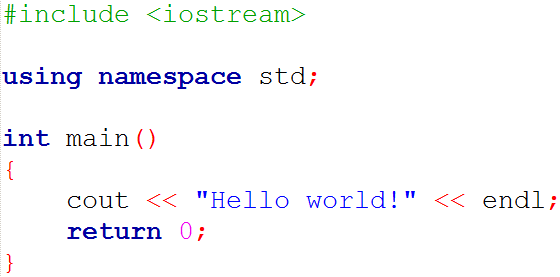
\includegraphics[width=\linewidth]{screenshots/c++_hello_world}
\caption{C++ print Hello world to console}
\label{fig:c++print}
\end{figure}
\begin{figure}
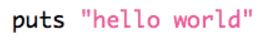
\includegraphics[width=\linewidth]{screenshots/ruby_hello_world}
\caption{Ruby print Hello world to console}
\label{fig:rubyprint}
\end{figure}
\par The above two images show C++ \ref{fig:c++print} and Ruby \ref{fig:rubyprint} printing ‘Hello world’ to the console. The comparison between the two languages highlights the efficiency and simplicity of the Ruby language.Ruby on Rails projects are commonly worked on by a group of people and in multiple languages, therefore the simplistic syntax gives greater clarity and understandability to programmers who are lesser experienced in Ruby.\cite{AboutRuby}
\par Ruby is open source, free and redistributable with a vast range of existing code from both Ruby and its large community. Primarily consisting of Gems, code packages that can be installed and supported into a project easily and with minimal effort via RubyGems, and frameworks, such as Ruby on Rails. Making it very popular for education and business. Following the DRY ‘Don't Repeat Yourself’ principle in a very effective and efficient manner.\cite{AboutRuby}
\par Ruby was ranked ninth on TIOBE index\cite{TOBIE} and has become a very popular and respected language relative to its age among the other languages on the index. No alternatives could be considered due to the dependency of Ruby on Rails on Ruby, however Ruby is a very strong and durable language so it does not detract from the overall project.
\par paragrpah about rails, more its specifics


\subsection{Testing and Automation}
\par The European Space Agency spent ten years and \$7 billion designing and constructing the Ariane 5, a rocket that can launch multiple satellites into orbit from a single launch. Thirty nine seconds into its maiden voyage it exploded, destroying the Ariane 5 and its contents of four uninsured, extremley expensive scientific satellites. The explosion was caused by its own self-destruct sequence which was triggered automatically as the boosters were being torn away by aerodynamic forces. The extreme aerodynamic forces were caused by the rocket trying to recorrect its course due to flight data provided the guidance system. The guidance system had crashed and shutdown, along with its backup, the flight data provided that caused the rocket to readjust its course was actually a diagnostic error message. The cause of the shutdown was the guidance system trying to convert the sideways velocity of the rocket from 64-bit to 16-bit where an overflow occured causing the system to shutdown. To make matters worse, the programmers were aware that it could overflow but assumed that particular variable would never be large enough as it was used to prepare for launch and not in flight. However it was decided the system should run into the first forty seconds of flight, incase of a brief hold in the launch countdown, to make restarting the system easier. A known flaw in a system, that could of been handled, ended up causing the chain of events that led to the rocket exploding.\cite{Ariane5}
\par Software testing is an investigation into a piece of software that provides information during development and maintenance. A process or series of process's are carried out that are designed to make sure computer code does what it designed to do and is absent of unintended behaviour. \cite{myers2011art}The information retrived from the proccess can be used to track the progress during development against acceptance criteria. Errors and bugs detected within the code of the are immediatley known and can be handled, providing a smoother and more consistent development and maintenance flow. Software testing provides a more reliable and higher quality product when used as part of the development process.
\par Testing can not guarantee that a program or peice of code is without errors, therefor completing testing is impossible. This is why the design of tests is vital to the integrity of the testing, making the tests as complete as possible. Given the constraints on time and cost, effective testing is simply "What subset of all possible test cases has the highest probability of detecting the most errors?"\cite{myers2011art}. Tests are designed using information about the program along with its intended behaviour. In a given environment, with proper determined input, there is an expected behaviour/output. If the code undertest does not display the desired outcome it is said to of failed the test. Design of tests is important and to design a test information is required, the information is sourced in two main ways Black Box and White Box.
\par Black box also known as Functional Testing is the technique of creating test cases with information from the software requirements and or its design specification. The software entity under test is treated as a black box where proper inputs are fed in and outputs are observed with no concern to the actual structure of the code. Black box testing can detect some behaviours that white box cannot, such as absent behaviours that are in the requirements but not coded in.\cite{nidhra2012blackbox}\cite{young2008software}
\par White box testing, structural testing uses information from the physical code to produce test cases. The derivation of information makes the test more focused on the actual implementation of the code rather than its specified behaviour. Test cases tend to be at a much finer grain than black box testing individual methods. Tests are designed to execute a particular behaviour within the program, such as testing how it handles a binary overflow.\cite{nidhra2012blackbox}\cite{young2008software}
\par As Ruby on Rails design environment can vary drastically between projects due to the flexibility of its framwork and use of Gems I will only consider Black Box testing techniues when I come to designing the project. This will deliver a product that will be usable to a wider audience as it is dependent upon on specification for which I can define. Interpreting multiple languages and being flexible enough to be useful is out of the scope of this project.
\par A 'test case' will test a very specific behaviour of a program. A collection of test cases is a 'test suite', representing that a certain section of the system has a specificied set of behavoiurs. A relevant example would be for a table in a database. The test suite would represent if the table has the desired validations in place and would consist of test cases that tested each specific behaviour in isolation. The tests would be run as a set to confirm the table has the desired behaviour, while being in the case of undesired behaviour being to specify which test case, therefore highlight the exact error in the code. Therefor to automate test generation, test cases need to be automatically generated with being able to identify the necessary cases to complete a set.
\par Software testing is necessary and very costly. "In a typical programming project approximately 50 percent of the elapsed time and more than 50 percent of the total cost were expended in testing the program or system being developed"\cite{myers2011art}. Reducing the costs, both time and monetary are the main motivations for Automated Testing. Another overlooked and unappreciated benefit of automating testing is test case generation is one the most intellectully demanding and critical challenges in software testing.\cite{anand2013orchestrated} By automating this process it allows the programmers to dedicate not only more time but more of thier effort to other areas, also in some cases it is harder to create a test case but easy to verify a generated test case is correct. A whole systems tests do not have to be automatically generated to reduce costs and benefit.
\par Automated functional testing follows the same method as manual generation of test cases. The information used to derive test cases is a functional specification: description of intented program behaviour distinct from the program itself. In manual this can be formal or informal, however in automated it is formal so that it can be interpreted by the system that will generate the test cases. The possible behaviours of the program derived from the formal specification are divided into test suites then again into test cases. For a database, tables would be divided into test suites, then as before the properties of the fields would be the test cases. The systematic nature can help avoid missed test cases and provide more consistent coverage. When automated there is more creativitivy and design put into the functional specification as the test designer is usually limited to a choice of test selection criteria.\cite{young2008software}
\par As observed with automated functional testing, a system is used to interpret and understand the same information that a human would use to produce test cases, effectively replacing the human user. Automated white box testing tends to be subsequently more complex, as it has to understand and interpret human written code. One method that has recieved alot of attention from researchers is Symbollic Execution, where symbollic values are used to instead of concrete values program inputs, the programs variables are then be described by the symbolic expressions of those inputs. The state of the program includes the symbolic values of program variables, a program counter and the path contraint on symbolic values: a boolean formula over the symbolic values input. Using this method it can explore all possible path divergences through a system and identify stop points, where the path ends. The major problem with automated white box testing is identifying if a behaviour, stop point or a specific divergence in Symbollic execution, is desired or not. This problem is known as the Oracle problem, as desired behavoiur of code is contained within its specfication and design, not its implementation. Therefor automated test generation must always include some level of user input. Another relevant challenge Symbolic Execution is developing a system that devloping system that can cover multiple languages at once is very complex and producing a system can produce feasible output can be impossible due to the path divergence problem, where either a user has to specify so many models it isn't automated wnough to benefit or it doesnt find a signifcant amount of feasible program paths.



\subsection{Testing in Rails}
\par various methods consistent models
\par test unit rspec
\par factory girl
\par rspec examples
\par suite example



\subsection{wrapup}
\par conclusion: research influenced project
	only model, black box, rspec, produce written tests etc etc

\subsection{Evaluation}
\par how testing is evaluated, code coverage bugs found etc
\par how other people tested, difficulties
\par maniuplation
\par dog feed
\par compare with existing
\par compare code coverage, how much of theres did it do
\par limited so not going to cover all, but does it save a signifacant amount of time



\section{Chapter 3: Requirements and Analysis}
Filler text, filler text, filler text, filler text, filler text, filler text, filler text, filler text.



\section{Chapter 4: Design}

\par front end - bootstrap - clean - easy to use

\par information required to generate test cases

\par how information should be entered

\par how information should be presented/edited

\par database design to accomadate the information

\par flow of program code to evaluate efficently

\par templates for rspec that can be filled in

\par generate button

\par number generation

\par string generation

\par output should be a file that is same as user created






\section{Chapter 5: Implemention and Testing}
Filler text, filler text, filler text, filler text, filler text, filler text, filler text, filler text.
\section{Chapter 6: Results and Discussion}
Filler text, filler text, filler text, filler text, filler text, filler text, filler text, filler text.
\section{Chapter 7: Conclusions}
Filler text, filler text, filler text, filler text, filler text, filler text, filler text, filler text.
Hello World!
\subsection{subsection}
Structuring a document is easy!! \cite{near2012rubicon}
\subsubsection{subsubsection}
\paragraph{p1}
It's a me, Mario\footnote{\label{myfootnote}\cite{near2012rubicon}}.
\subparagraph{sp1}
Wwoohooo
\section{image}
\begin{figure}
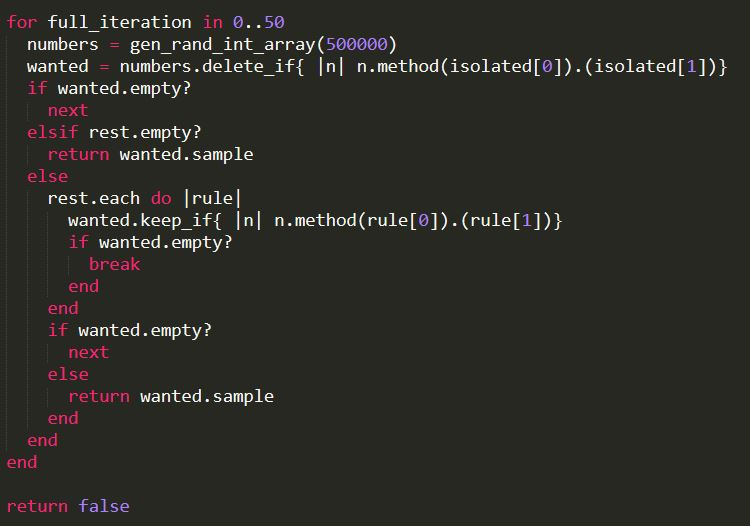
\includegraphics[width=\linewidth]{screenshots/code-gen-int-pre_divisible_keep_if}
\caption{caption for image, shown below image}
\label{fig:code1}
\end{figure}
Figure \ref{fig:code1} shows some savage code

	
\begin{table}[h!]
\centering
\caption{Caption for the table.}
\label{tab:table1}
\begin{tabular}{ccc}
\toprule
Some & actual & content\\
\midrule
prettifies & the & content\\
as & well & as\\
using & the & booktabs package\\
\bottomrule
\end{tabular}
\end{table}

\bibliography{bibliography}
\bibliographystyle{ieeetr}
\end{document}
